\chapter{Lake Macalania}

\begin{enumerate}
	\item Run up and \sd
\end{enumerate}
\begin{battle}[16000]{Crawler}
	\begin{itemize}
		\switch{\tidus}{\rikku}
		\rikkuf Lightning Marble x1/2 Negator (1\,000 HP)
		\rikkuf Lightning Marble Crawler
		\kimahrif Lightning Marble Crawler
		\luluf Phoenix Down \rikku
		\ifthenelse{%
		\equal{\blitzresult}{win}}{%
			      \switch{\kimahri}{\yuna} \textit{If \kimahri\ didn't die}
			      \yunaf Defend
			      \rikkuf Lightning Marble Crawler
			      \luluf Phoenix Down \rikku\ \textit{If \kimahri\ didn't die else} Swap for \yuna\ and \yuna\ Phoenix Down \rikku
		}{\ifthenelse{\equal{\blitzresult}{loss}}{%
		\item \textit{If you have a Lunar Curtain:}
		      \begin{itemize}
			      \switch{\kimahri}{\yuna} \textit{If \kimahri\ didn't die}
			      \yunaf Defend
			      \rikkuf Lightning Marble Crawler
			      \luluf Phoenix Down \rikku\ \textit{If \kimahri\ didn't die else} Swap for \yuna\ and \yuna\ Phoenix Down \rikku
		      \end{itemize}
		      \item \textit{If you don't have a Lunar Curtain:}
		      \begin{itemize}
			      \kimahrif Steal
			      \rikkuf Lightning Marble Crawler
			      \switch{\lulu}{\yuna}
			      \yunaf Phoenix Down \rikku
		      \end{itemize}
		}{\ifthenelse{\equal{\blitzresult}{both}}{%
		\item \textit{If \blitzwin\ or you have a Lunar Curtain:}
		      \begin{itemize}
			      \switch{\kimahri}{\yuna} \textit{If \kimahri\ didn't die}
			      \yunaf Defend
			      \rikkuf Lightning Marble Crawler
			      \luluf Phoenix Down \rikku\ \textit{If \kimahri\ didn't die else} Swap for \yuna\ and \yuna\ Phoenix Down \rikku
		      \end{itemize}
		      \item \textit{If \blitzloss\ and don't have a Lunar Curtain:}
		      \begin{itemize}
			      \kimahrif Steal
			      \rikkuf Lightning Marble Crawler
			      \switch{\lulu}{\yuna}
			      \yunaf Phoenix Down \rikku
		      \end{itemize}
		}{}}}
		
		      \switch{\yuna}{\tidus}
		      \tidusf Defend
		      \rikkuf \od, HP Sphere and Lightning Marble
	\end{itemize}
	\tidus, \yuna, \lulu\ need AP.
\end{battle}
\bothvfill
\winvfill
\lossvfill
\begin{spheregrid}
	\begin{itemize}
		\tidusf (22 S.Lvl)
		\begin{itemize}
			\item Level 2 Key Sphere
			\item Move $\rightarrow\uparrow$
			\item Str +4
			\item Move $\uparrow\uparrow$
			\item HP+200
			\item Move $\rightarrow\rightarrow\uparrow$
			\item HP+200, Str+4, Agi+2
			\blitzballdetermination[true]{%
				      \item Move $\rightarrow$
				      \item Use Strength Sphere, Activate it
				      \item Move $\uparrow\leftarrow\leftarrow$ or $\nwarrow\nwarrow$
			}{%
				      \item Move $\uparrow\nwarrow$			
			}
			\item HP+200, Str+4, Agi+2
			\item Move $\leftarrow$
			\item Str+4
		\end{itemize}
		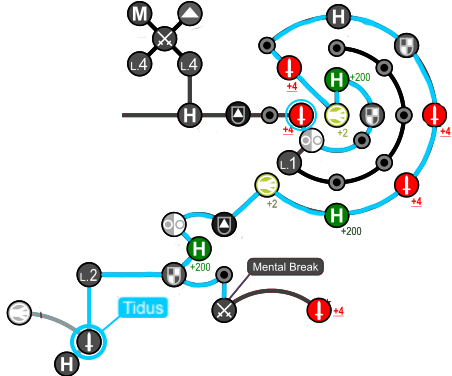
\includegraphics[width=.8\columnwidth]{graphics/Tidus_post_crawler}
	\end{itemize}
\end{spheregrid}
\begin{enumerate}[resume]
	\item Tidus should have 1320 Max HP
	\item \sd, \cs[0:40], head to next screen
	\item Head to Temple, \sd. \save, speak to Tromell for \textbf{Shell Targe}
	\item Jyscal Skip:
	      \begin{itemize}
		      \item Walk into the wall to the right of Tromell
		      \item Move slightly to the right, turn around and Talk to Tromell while moving Right.
		      \item If successful, walk forward while mashing Shelinda's dialogue.
		      \item When dialogue finishes, walk up the stairs, push the man, and go through.
		      \item If Shelinda is not saying her dialogue, talk to one of the musicians
	      \end{itemize}
	\item \sd, walk to Fayth room, \cs[2:10]
\end{enumerate}
\bothvfill
\begin{battle}[3000]{Seymour}
	\begin{itemize}
		\blitzballdetermination[true]{%
			      \tidusf Switch to Brotherhood
			      \tidusf Haste \tidus
			      \enemyf Seymour Blizzara
			      \tidusf Talk to Seymour
			      \yunaf Change Weapon Staff to Staff
			      \enemyf Guado Guardians None/Blizzard/Thunder/Shremedy
			      \kimahrif Defend. If Shremedy landed, Remedy/Attack the afflicted target. If \yuna\ is dead, Phoenix Down
			      \switch{\yuna}{\auron}
			      \auronf Defend
			      \tidusf \od\ Spiral Cut Seymour
			}{%
		      		\tidusf Haste \tidus
			      \tidusf Cheer
			      \tidusf Talk to Seymour
			      \yunaf Change Weapon
			      \switch{\kimahri}{\rikku}
			      \rikkuf Defend. If Shremedy landed, Remedy the afflicted target.
			      \switch{\yuna}{\kimahri}
			      \kimahrif Defend. If Shremedy landed, Remedy the afflicted target.
			      \tidusf Switch to Brotherhood
			      \tidusf \od\ Spiral Cut Seymour
			}
	\end{itemize}
\end{battle}
\bothvfill
\lossvfill
\begin{battle}[18000]{Anima}
	\begin{itemize}
		\blitzballdetermination[true]{%
			      \switch{\tidus}{\wakka}
			      \wakkaf Change Weapon
			      \kimahrif Steal
			      \enemyf Pain
			      \switch{first survivor}{\tidus}
			      \tidusf Attack x4
			      \switch{second survivor}{\rikku}
			      \rikkuf Steal/Phoenix Down \yuna\ if she's dead
			}{%
			      \rikkuf Use Lightning Marble/Bomb Core/Arctic Wind
			      \switch{\tidus}{\wakka}
			      \wakkaf Change Weapon
			      \kimahrif Use Lightning Marble/Bomb Core/Arctic Wind
			      \enemyf Pain
			      \switch{\wakka}{\tidus}, if \wakka\ died then switch \rikku\ instead.
			      \tidusf Attack x4
			      \switch{\kimahri}{\rikku} \textit{if you had to switch out \rikku\ before}
			      \rikkuf Steal/Phoenix Down \yuna\ if she's dead.
		      }
		      \tidus\ and \yuna\ need AP.
	\end{itemize}
\end{battle}
\begin{battle}[6000]{Seymour}
	\begin{itemize}
		\tidusf Defend x2 until Multi-Thundara, Phoenix Down \rikku\ if she died before Multi-Thundara.
	      \rikkuf Defend
	      \tidusf Attack x2
	\end{itemize}
\end{battle}
\begin{enumerate}[resume]
	\item Name \shiva
\end{enumerate}
\begin{equip}
	\begin{itemize}
		\tidusf Sonic Steel
	\end{itemize}
\end{equip}
\winvfill
\begin{spheregrid}
	\begin{itemize}
		\tidusf
		\begin{itemize}
			\item Move $\leftarrow\leftarrow$
			\item HP+200
			\item Move $\leftarrow\uparrow\uparrow$
			\item Str+4, Agi+2
		\end{itemize}
		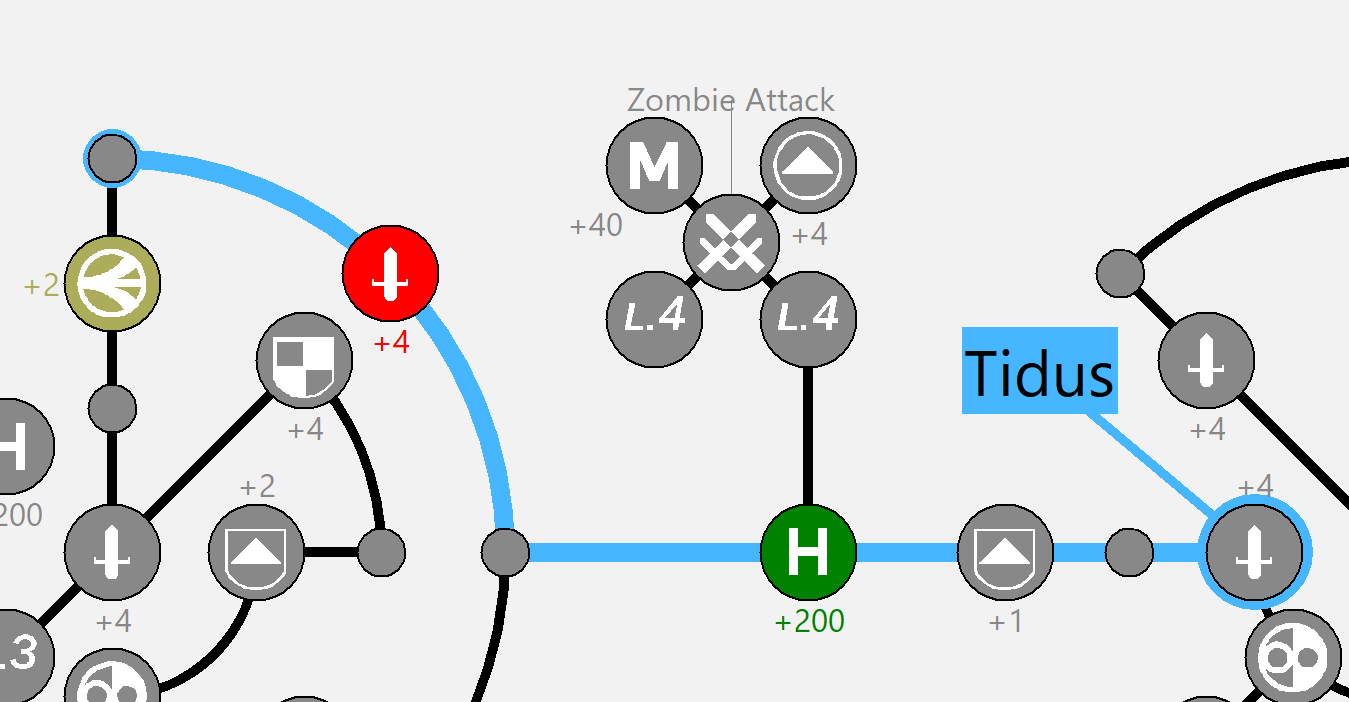
\includegraphics[width=.8\columnwidth]{graphics/Tidus_Post_Seymour}
	\end{itemize}
\end{spheregrid}
\begin{enumerate}[resume]
	\item \formation{\rikku}{\tidus}{\yuna}
\end{enumerate}
\begin{trial}
	\begin{itemize}
	  \item \save, exit Fayth room.
	  \item Slide pedestal to the right
        \item Take sphere from the right wall, place into pedestal
        \item Push pedestal up
        \item Take Glyph sphere from middle pillar
        \item Go downstairs and push pedestal to the right
        \item Place Glyph sphere in far left slot in the wall
        \item Go upstairs, pick up new sphere
        \item Go downstairs, place sphere in pillar
        \item Go upstairs, take the sphere at the top of the slope
        \item Place in last pillar
	\end{itemize}
\end{trial}
\begin{enumerate}[resume]
	\item Go to temple entrance, \sd
	\item Move south and go down the left path.
	\blitzballdetermination[true]{}{\item Do at least one of the Guado Encounters.}
\end{enumerate}
\begin{encounters}
	\begin{itemize}
		\item Guado Fight:
		      \begin{itemize}
			      \tidusf Attack Guado, then Surviving Enemies
			      \rikkuf Silence Grenade
			      \yunaf Defend
		      \end{itemize}
	\end{itemize}
\end{encounters}
\blitzballdetermination{}{
\begin{spheregrid}
	\begin{itemize}
		\tidusf Move $\downarrow\downarrow$
		\item Str+4
	\end{itemize}
	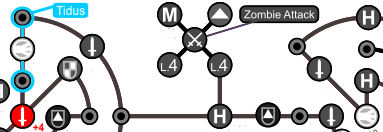
\includegraphics[width=.8\columnwidth]{graphics/tidus_bikanel}
\end{spheregrid}}
\bothvfill
\begin{battle}[18000]{Wendigo}
	\begin{itemize}
		\tidusf Haste \tidus
		\tidusf Switch Weapon to Brotherhood
		\tidusf Attack Guado B (Top One)
		\item \textit{If Light Curtain:}
		      \begin{itemize}
			      \rikkuf Light Curtain \tidus
		      \end{itemize}
		      \textit{Else:}
		      \begin{itemize}
			      \switch{\rikku}{\auron}
			      \auronf Power Break
		      \end{itemize}
		      \tidusf Attack Wendigo until its dead, then Guado
		      \yunaf Defend/Elixir \tidus/Phoenix Down Dead Ally
		      \rikkuf Defend/Elixir \tidus/Steal Guado/Phoenix Down Dead Ally
		      \switch{\yuna}{\lulu}
	\end{itemize}
	\yuna, \tidus\ need AP. Helpful if \lulu\ gets it.
	Guaranteed 2 Power Spheres.
\end{battle}
\begin{enumerate}[resume]
	\item Run up to \rikku, \sd, walk up to \yuna, \sd, \save, run past \kimahri\ and go to the hidden area to \pickup{Level 2 Key Sphere}
	\winvfill
	\item Run up to \auron\ and speak with him, \sd, walk back, \cs+\skippablefmv[1:00], (press Start immediately after skip), \sd\ in Dream Sequence
\end{enumerate}